
\documentclass[12pt,a4paper]{article} % Use A4 paper with a 12pt font size - different paper sizes will require manual recalculation of page margins and border positions

% Generated with LaTeXDraw 2.0.8
% Mon Jun 17 19:00:40 EDT 2013
\usepackage[usenames,dvipsnames]{pstricks}
\usepackage{epsfig}
\usepackage{pst-grad} % For gradients
\usepackage{pst-plot} % For axes
%\usepackage{marginnote} % Required for margin notes
%\usepackage{wallpaper} % Required to set each page to have a background
%\usepackage{lastpage} % Required to print the total number of pages
\usepackage[left=1.3cm,right=4.6cm,top=1.8cm,bottom=4.0cm,marginparwidth=3.4cm]{geometry} % Adjust page margins
\usepackage{amsmath} % Required for equation customization
\usepackage{amssymb} % Required to include mathematical symbols
\usepackage{xcolor} % Required to specify colors by name
\usepackage{amsthm}
\usepackage{float}


\setlength{\parindent}{0cm} % Remove paragraph indentation
\newcommand{\tab}{\hspace*{2em}} % Defines a new command for some horizontal space


\title{Calculus and Workshop - Optimization Unit}
%----------------------------------------------------------------------------------------

\newtheorem{defn}{Definition}
\newtheorem{example}{Example}
\newtheorem{prop}{Proposition}
\newtheorem{exer}{Exercises}
\newtheorem{thm}{Theorem}
\begin{document}
\maketitle

\section{Optimization of Functions}
One of the most important applications of differential calculus is the 'optimization' of functions, where 'optimization' means finding out where a function is either maximized (has its greatest value) or minimized (has its smallest value).  These values are called 'extrema'.  \\\\
There are two types of extrema: Global and local.  'Global' means we look for an 'extreme value' (max or min) over the entire domain of the function.  'Local' means that we consider the extreme values of a function within a subset of the domain.  This nomenclature can cause some confusion, as we sometimes consider optimization over a closed interval that is a subset of the domain to be 'global' - in this case, 'global' means over the interval being considered.  Let's consider the procedure for locating extreme values and then we will clarify this.\\\\

Recall that the \emph{critical points} of a function $f$ are the values where its derivative $f'$ vanishes.  Geometrically, these are the points at which the tangent line is horizontal (it has zero slope).  This indicates a possible point where the derivative may be changing sign, and therefore the function would be changing from increasing to decreasing or vice-versa.  If the slope is changing sign, such a point is a local max or min.  \\\\

If we are considering a function on a closed interval, we must also check the endpoints of the interval.  If we find that the function when evaluated at either of the endpoints has values that are larger than the max (or smaller than the min), then the max (min) is at the endpoint.  Otherwise, we conclude that the max (min) over the interval is at the critical point.  Now - we may say that the max (min) of our function is a 'global' max (min) \emph{over the interval}.  It is possible that when we consider the entire domain, our max (min) is actually local (i.e. there could be a more extreme point, or the function may not have a max or min over the entire domain).  In other words, we need to be careful with our notion of 'global'. Consider the following illustrations:
\begin{figure}[H]
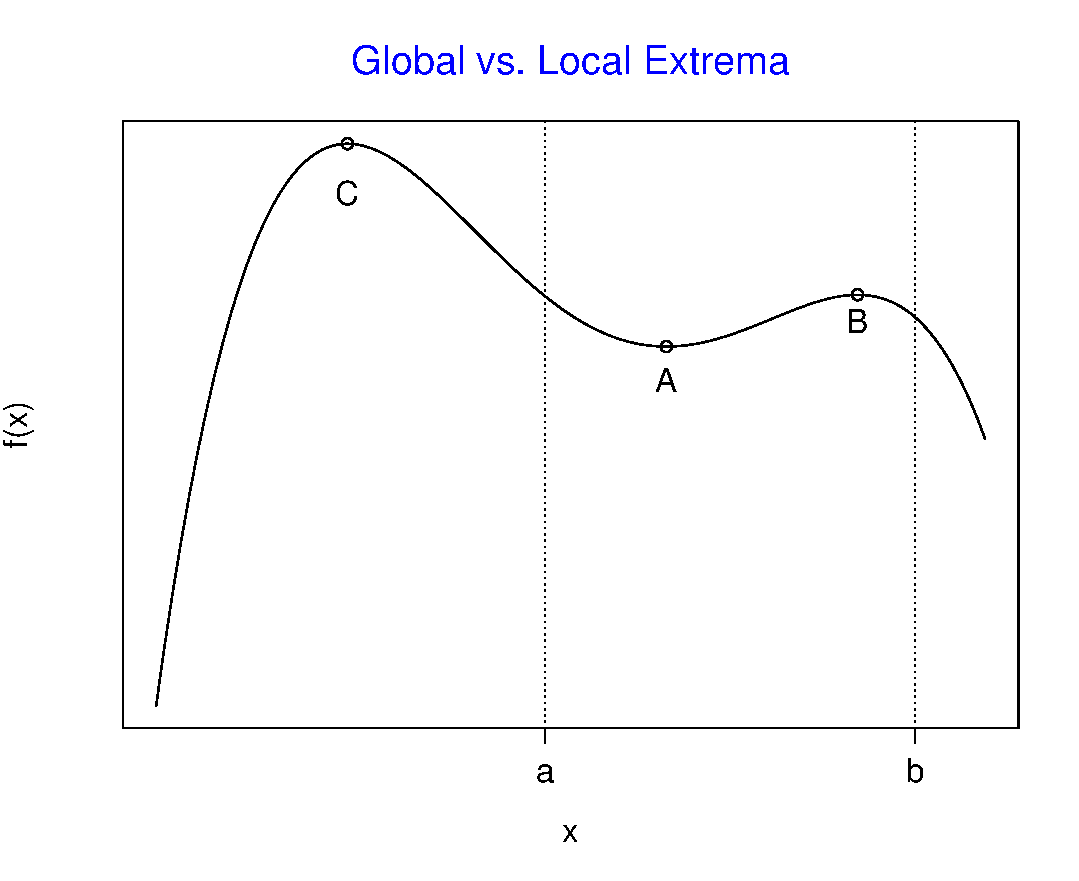
\includegraphics[height=3in]{Extrema1.pdf}
\caption{Global vs. Local Extrema.  This is the graph of a fourth degree polynomial, $f(x)= -30x + (11x^2)/2 + (4x^3)/3 - x^4/4$.   On the interval $[a,b]$, this function has a global minimum at point $A$ and a global maximum at point $B$.  Over the entire domain, this function has a global maximum at point $C$ and no global minimum - the points $A$ and $B$ are a local minimum and maximum respectively.}
\end{figure}
\begin{figure}[H]
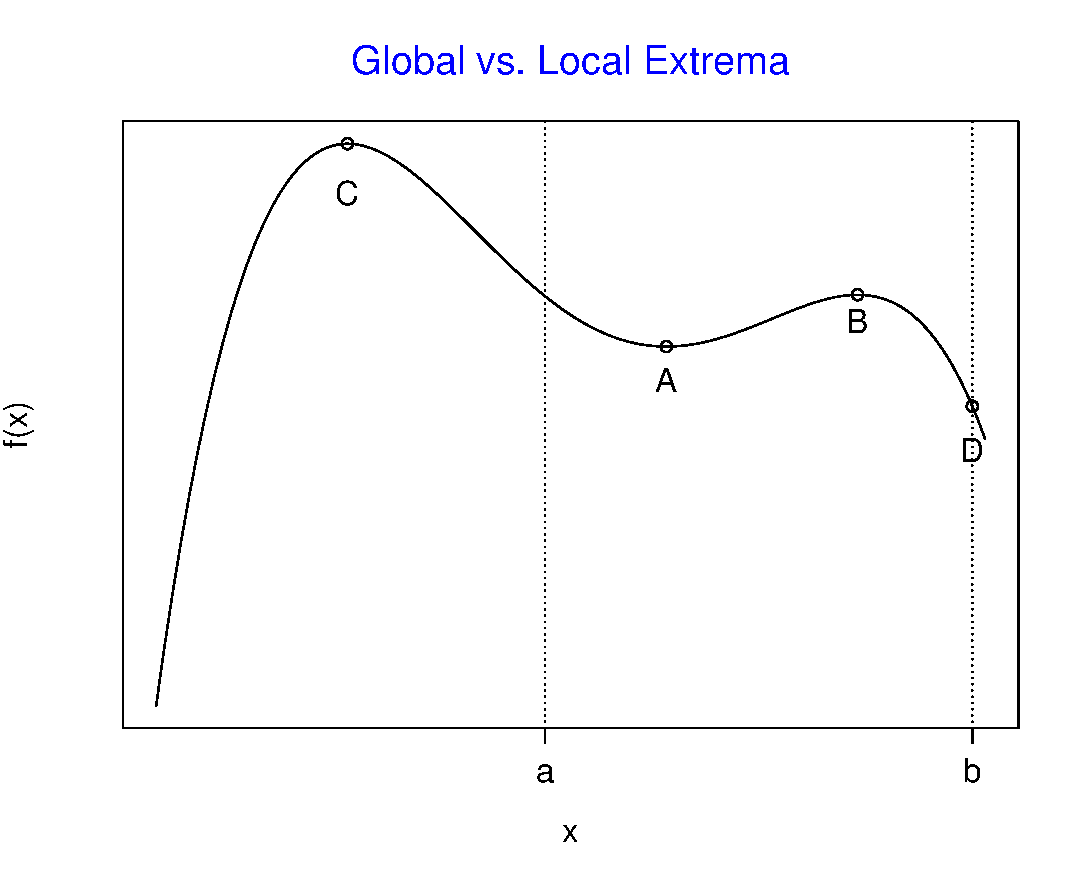
\includegraphics[height=3in]{Extrema2.pdf}
\caption{Global vs. Local Extrema.  We consider the same function as in the previous figure, but over a slightly different interval.  We can see from the graph that the global minimum over the interval $[a,b]$ occurs at the endpoint $b$.  The global maximum is at point $B$, and $A$ is a local minimum.}
\end{figure} 
\subsection{Characterizing Max and Min}
Suppose we have a function $f(x)$, and we have found $f'(x)$, set it to zero and found some critical points. How do we know whether we have a max or a min at that point? \\

We can note that the sign of the derivative at a point tells us whether the function is increasing or decreasing at that point. If we take the derivative of $f'(x)$, (that would be $f''(x)$) we can determine whether $f'(x)$ is increasing or decreasing. \\

Now, at the critical point, $f'(x)$ is zero. So, if the critical point is a max or a min, $f'(x)$ is changing sign - either negative to positive (increasing, $f'' >0$) or positive to negative (decreasing, $f'' <0$). In the first case, we have a minimum, in the second case, a max. This is known as the 'second derivative test'.\\

If the second derivative is zero at the critical point, the second derivative test fails. In this case, we can use the 'first derivative test', where we directly test for a change in sign of the first derivative around the critical point. \\

Consider the functions $f(x) = x^4$ and $f(x) = x^3$. Both have a singular critical point at $x = 0$, but the second derivative also vanishes at $x=0$. Plot these functions and examine what is happening with the first derivative around the critical point. what is the difference in behavior?\\

\begin{exer}
Characterize extrema for the following:

\begin{enumerate}
\item 
$$f(x) = x^2, \;\;\;\;\;\;\;\textrm{ on the interval } [-1,2]$$

\item 
$$f(x) = x^3 + 2, \;\;\;\;\;\;\;$$

\item 

$$-6 x + \frac{17 x^2}{2} - \frac{14 x^3}{3} + \frac{3 x^4}{4}$$
\end{enumerate}

\end{exer}

\newpage
\subsection{Monotone Functions}
A class of functions that is often useful to us in analysis is the class of \emph{monotone} functions.  A monotone function is simply a function that doesn't 'go up and down' (think of a monotone voice).  Formally:
\begin{defn}
A function $f(x)$ is said to be \emph{monotonically increasing} if
$$f(x_2) > f(x_1)$$
whenever
$$x_2 > x_1$$ 
Conversely, if 
$$f(x_2) < f(x_1)$$
whenever
$$x_2 > x_1$$
$f(x)$ is said to be \emph{monotonically decreasing} 
\end{defn}
When the inequalities are not strict, we say that $f(x)$ is \emph{monotonically non-decreasing} or \emph{monotonically non-increasing}, respectively. \\\\
 It is easy to see that a function $f(x)$ is monotonically increasing $\iff f'(x)\geq0$ for all $x$, and $f(x)$ is monotonically decreasing $\iff f'(x)\leq0$ for all $x$.   
\begin{example}
$\log(x)$ is monotonically increasing on the interval $(0,\infty)$. 
\end{example}
\begin{proof}
$$\frac{d}{dx}\log(x) = \frac{1}{x} > 0 \;\;\;\;\;\;\mathrm{for all }\;\; x\in(0,\infty)$$
\end{proof}
\subsection{Monotone Functions and Optimization}
Monotone functions have an important property with respect to optimization: we can compose a monotone function with a function of interest without changing the location of extrema.  Often, we will use the monotone function $\log(x)$. Recall that $\log$ has the property that:
$$\log(xy) = \log(x) + \log(y)$$
Suppose we have a function of the form:
$$f(x) = h_1(x)h_2(x)h_3(x)...h_n(x)$$
In other words, $f$ is the product of $n$ functions.  If we want to find the critical values of this function, we could differentiate using the product rule - but that would be messy and we would probably make some kind of error in the process.  Now, if we take the $\log$:
$$\log(f(x)) = \log(h_1(x)h_2(x)h_3(x)...h_n(x))$$
$$= \log(h_1(x))+ \log(h_2(x))+\log(h_3(x))+...+\log(h_n(x))$$
Now, we can differentiate a sum instead of a product.  This is a whole lot easier.  We also note, that by the chain rule:
$$\frac{d}{dx}\log(f(x)) = \frac{1}{f(x)}\frac{d}{dx}f(x)$$
and so we have
$$\frac{d}{dx}\log(f(x)) = \frac{1}{h_1(x)}\frac{d}{dx}h_1(x)+...+\frac{1}{h_n(x)}\frac{d}{dx}h_n(x)$$

\end{document}